\documentclass[12pt,fleqn]{article}
\usepackage[margin=1in,top=1in,bottom=1in]{geometry}
\usepackage{mathtools}
\usepackage{longtable}
\usepackage{enumitem}
%\usepackage{hyperref}
\usepackage[dvips]{graphics}
\usepackage[table]{xcolor}
\usepackage{amssymb}
\usepackage{float}
\usepackage{booktabs}
\usepackage{tikz}
\usepackage{subcaption}
\usepackage{wrapfig}

\usepackage[normalem]{ulem}

\usepackage{multicol}
\usepackage{txfonts}
%\usepackage{amsfonts}



%%%%%%%%%% bibliography stuff %%%%%%%%%%%%%
%\usepackage[numbers]{natbib}
%\bibliographystyle{abbrvnat}
\usepackage{natbib}
\bibliographystyle{/Users/tonhauser.1/Library/Latex/cslipubs-natbib}

\setlength{\bibhang}{0.5in}
\setlength{\bibsep}{0mm}
\bibpunct[:]{(}{)}{;}{a}{,}{,}
%%%%%%%%%%%%%%%%%%%%%%%%%%%%%%%

\usepackage{wrapfig}
%\setlength{\intextsep}{8pt}%
\setlength{\columnsep}{8pt}%

\usepackage{gb4e}
%\usepackage{/Users/judith/Library/Latex/drs}
%\usepackage{/Users/judith/Library/Latex/avm}
\usepackage[all]{xy}
\usepackage{rotating}
\usepackage{tipa}
\usepackage{multirow}
\usepackage{authblk}
\usepackage{adjustbox}
\usepackage{array}

\usepackage{titlesec}
\titleformat*{\section}{\bfseries\footnotesize}
 
\setlength{\parindent}{.3cm}
\setlength{\parskip}{0ex}

\renewcommand\figurename{Fig.}

\newcommand{\yi}{\'{\symbol{16}}}
\newcommand{\nasi}{\~{\symbol{16}}}
\newcommand{\hina}{h\nasi na}
\newcommand{\ina}{\nasi na}

\exewidth{(\thexnumi)}

\newcommand{\citepos}[1]{\citeauthor{#1}'s \citeyear{#1}}
\newcommand{\citetpos}[1]{\citeauthor{#1}'s (\citeyear{#1})}

\newcommand{\6}{\mbox{$[\hspace*{-.6mm}[$}} 
\newcommand{\9}{\mbox{$]\hspace*{-.6mm}]$}}
\newcommand{\sem}[2]{\6#1\9$^{#2}$}
\renewcommand{\ni}{\~{\i}}

\newcommand{\jt}[1]{\textbf{\color{blue}JT: #1}}


\setlength{\belowcaptionskip}{-10pt}


 \begin{document}
  
\begin{center}
{\bf Higher-probability content is more projective than lower-probability content}
\\ Judith Tonhauser (Ohio State U / Stuttgart U) \& Judith Degen (Stanford U)
\end{center}

\vspace*{-.3cm}

\noindent
A hallmark of the content of the complement (CC) of factive predicates like {\em know}  is that it projects. For example, in an utterance of the sentence \emph{Does Jane know that Sam has a new hat}, the speaker is typically taken to be committed to Sam having a new hat, despite the predicate and the CC being embedded under an entailment-canceling operator (the polar interrogative). The same is typically not true when replacing \emph{know} with a non-factive predicate like \emph{think}. However,  \citealt*{tbd-variability} ({\em Journal of Semantics}) recently showed that there is substantial variability in the projectivity of CCs. While a lot of this variability was explained by the not-at-issueness of the CC, they also found that the lexical content of the CC played a role: e.g., the CC \emph{Sam has a new BMW} was less likely to project than \emph{Sam has a new hat}. The authors hypothesized that the projectivity of a CC may depend on its prior subjective probability, such that a CC is more projective the higher its prior probability. The current work finds support for this hypothesis in an experimental investigation of CCs of both factive and non-factive predicates in which the prior probability of the CC was systematically manipulated. We argue that this finding provides support for constraint-based projection analyses that derive the projectivity of utterance content from the integration of multiple cues, including prior CC probability and the meanings of clause-embedding predicates.


\noindent
{\bf Prior probability norming experiment (n = 95).} Prior probability was measured for 20 contents denoted by English sentences (e.g., Julian dances salsa) given a fact that made the content more likely (e.g., Julian is from Cuba) and a fact that made it less likely (e.g., Julian is from Germany). Participants were asked how likely a content is given a fact (e.g., Fact: Julian is from Cuba. How likely is it that Julian dances salsa?) and provided ratings on a sliding scale from `impossible' (interpreted as a probability of 0) to `definitely' (interpreted as a probability of 1). The mean ratings were .7 for high- and .16 for low-probability contents, see Fig.~\ref{f-prior} for the full set of items.

\noindent 
{\bf Projectivity experiment (n=300).} The 20 sentences denoting the normed contents were realized as the complements of 20 clause-embedding predicates, for a total of 400 predicate/complement combinations. These combinations were realized as polar questions with a random subject noun phrase. In the target stimuli, the 400 polar questions were combined with one of the two facts that each content was normed with, for a total of 800 target stimuli. As shown in the sample target stimulus in (\ref{stim}), the named speaker (here, Carol) was explicitly stated to be aware of the fact.
\vspace*{-.6cm}
\begin{wrapfigure}{r}{.31\paperwidth}
\centering
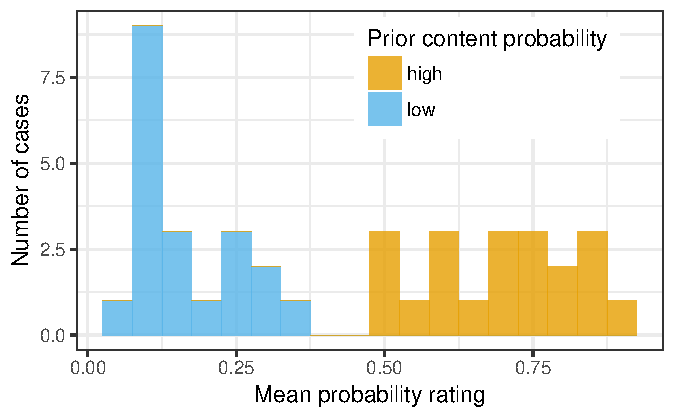
\includegraphics[width=.32\paperwidth]{../results/1-prior/graphs/meanprobratings}
\caption{Histogram of mean prior probability ratings for each item (i.e., content/fact combination). Color indicates whether item was coded as high or low probability in the projectivity analysis.}\label{f-prior}
\end{wrapfigure}%
\begin{exe}
\ex\label{stim}
{\bf Fact (which Carol knows):} Julian is German.  \\ 
{\bf Carol:} Does Sandra know that Julian dances salsa?
\end{exe}
\vspace*{-.15cm}
The 20 predicates included the 5 factives {\em be annoyed, know, see, discover} and {\em reveal}, as well as 15 non-factives: the CC of 9 of these ({\em acknowledge, admit, announce, confess, confirm, establish, hear, inform, prove}) has been described as being able to project (e.g., \citealt{schlenker10,anand-hacquard2014,spector-egre2015,tbd-variability}), in contrast to that of the remaining 6 predicates ({\em pretend, suggest, say, think, be right, demonstrate}).



\noindent Projectivity was measured with the `certain that' diagnostic, following \citealt{tbd-variability}: for (\ref{stim}), participants judged whether Carol is certain that Julian dances salsa. Participants rated 20 target items (one for each predicate) and 6 control items (as attention checks). They responded on a sliding scale from `no' (no projection, coded 0) to `yes' (maximal projection, coded 1).
\begin{wrapfigure}{l}{.45\paperwidth}
\centering
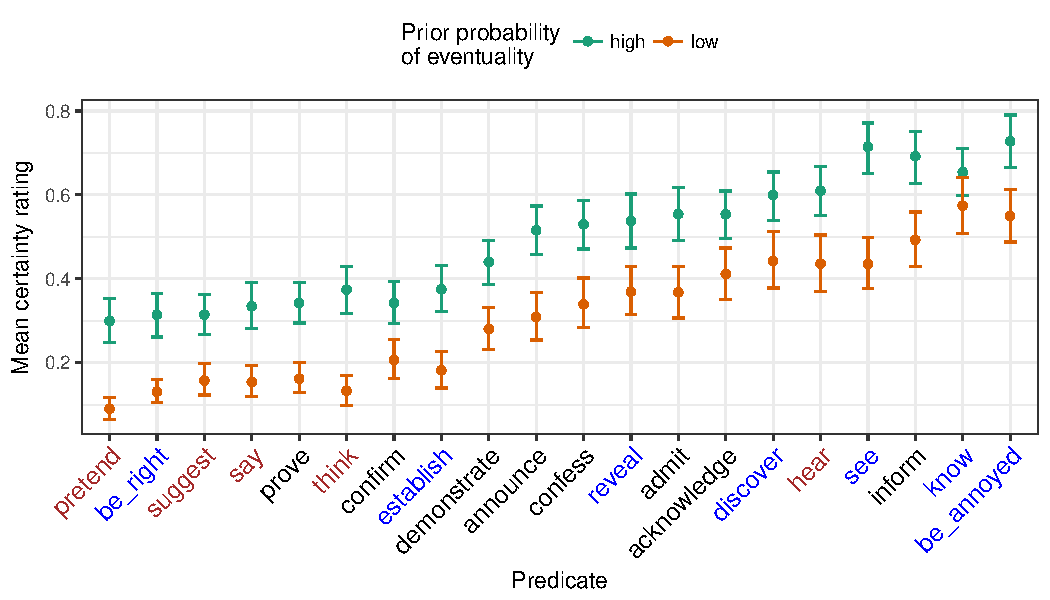
\includegraphics[width=.45\paperwidth]{../results/3-projectivity/graphs/means-projectivity-by-predicate-and-facttype}
\caption{Mean certainty rating by predicate (x-axis) and prior CC probability, with 95\% CIs; factives in green.}\label{f-proj}
\end{wrapfigure}

\noindent
{\bf Results.} As shown in Fig.~\ref{f-proj}, mean certainty ratings for CCs were higher when the content had a higher prior probability than when it had a lower prior probability, as hypothesized by \citet{tbd-variability}. Furthermore, the effect of prior CC probability on projectivity was present across all 20 predicates, factive and non-factive ones. We also observe by-predicate variability in mean certainty ratings:  e.g., the means for factive {\em be annoyed} were higher, at .72 (high) / .53 (low), than those for factive {\em reveal}, at .55 / .37, which were higher than those for non-factive {\em establish}, at .39 / .19. These findings replicate \citetpos{tbd-variability} finding that projectivity is a gradient property of utterance content.

A linear mixed-effects model predicting certainty rating from prior probability (high vs.\ low) and verb (reference levels: low prior probability, {\em pretend}) with random intercepts for participant and item and a random by-participant slope for prior probability revealed a significant main effect of prior probability ($\beta$ = .19, SE = .01, t = 13.39, $p <$ .0001) and significantly higher certainty ratings for all predicates except for {\em be right} and {\em suggest} (5520 data points). A model that included an interaction term for the fixed effects was not significantly better than the model reported here.

\noindent
{\bf Discussion.}
These results support \citetpos{tbd-variability} hypothesis that prior content probability influences projectivity. The finding that the CC of many non-factive predicates is at least weakly projective, even with low prior probability CCs, confirms intuitions reported in, e.g., \citealt{schlenker10}, \citealt{anand-hacquard2014} and \citealt{spector-egre2015}. These findings motivate the development of projection analyses that derive the influence of prior content probability and make predictions for the CCs of a broad range of both factive and non-factive predicates.

Current projection analyses, while limited to the CCs of factive predicates (e.g., \citealt{heim83,vds92,abrusan2011,brst-salt10,brst-ar}), are compatible with the finding that prior content probability influences projectivity. \citealt{heim83}, for instance, assumes default global accommodation when a presupposition is not entailed by the common ground (CG) when the trigger is uttered. This default is overridden when the presupposition is inconsistent with the CG. If we can assume that Julian dancing salsa is more likely to be consistent with the CG when Julian is from Cuba than when he is from Germany, \citealt{heim83} predicts that the presupposition that Julian dances salsa is more projective when it has a higher prior probability. 

As shown in Fig.~\ref{f-proj}, the CCs of several non-factives, including {\em inform, hear, acknowledge} and {\em admit}, are at least as projective as that of factive {\em reveal}. This finding challenges the long-standing assumption that the CCs of factives are more projective than those of non-factives. We suggest that this motivates constraint-based analyses that derive the projectivity of utterance content from the integration of multiple cues, including prior CC probability, the meanings of clause-embedding predicates, at-issueness (\citealt{tbd-variability}), and information structure (\citealt{tonhauser-salt26}).

\end{document}

\newpage

\bibliography{../bibliography}

\end{document}
